\documentclass{article}

\title{Measuring Red Algae in the Santa Ana River}
\author{EA30: Valeria Sanchez-Jimenez, Frank Lyles, Olivia Howie} 

\usepackage{Sweave}
\begin{document}
\Sconcordance{concordance:Tuesday_1_Report_Outline.tex:Tuesday_1_Report_Outline.Rnw:%
1 81 1 49 0 4 1 4 0 6 1 27 0 14 1 6 0 6 1 6 0 4 1 6 0 4 1 6 0 19 1}



\maketitle

\newpage
\tableofcontents
\newpage

\section{Introduction}


\subsection{Problem Statement}

The abundance of the red algae (\emph{Cosmopogen aeruginosus}) has recently risen significantly in the Santa Ana River. In a similar time period, the Santa Ana Sucker (\emph{Catostomus santaanae}), an endangered fish endemic to this and another three rivers in the Southern California region, has been experiencing population declines. This experiment explores the change in red algae presence in the Santa Ana River and the possible relationship it holds with Santa Ana Sucker's decline. Using measurments of river water temperature, overhead tree canopy cover, and sediment type we explore the connection these aspects of the river and their relationship with the red algae.

\subsection{Background Research} 
This project is motivated by the decline of the threatened Santa Ana sucker, a small freshwater sucker fish endemic to southern California, where it is now present in only three rivers. While there are several threats to the Santa Ana sucker, including fragmentation of its river habitats and decreasing water levels and degradation to the riparian vegetation along the river (Thomson 2010), red algae presence has significantly increased at this same time that the Suckers are dying. For the Santa Ana River sucker habitat, a central threat is the invasive Red Algae that has been spreading with alacrity in areas where the fish are known to be, including the reach below the Rapid Infiltration and Extraction (RIX) Treatment plan (Los Huertos 2016).There are concerns that it may be one of the contributing factors to the suckers decline. This project therefore focuses on qualitatively identifying and analyzing the substrate on which the red algae grows, because one of the aspects of the suckers habitat is the presence of coarse substrate, that is, gravel and cobble, as opposed to silt and sand (Thomson et al. 2010, 321). The sucker has adapted to feeding on the diatoms that tend to grow on the former. There is also evidence that some of the diatoms on which the sucker feeds may be able to grow on the algae (are epiphytic) (Los Huertos 2016). This may lead to the sucker being in contact with the algae when feeding. If the sucker is ingesting the algae, this may constitute a factor to the Suckers decline. Of course, ingesting the algae is not a necessity to the fish being negatively impacted; the algae may also disrupt the fishs well-being in unknown ways. Some researchers suggest that it actually crowds out the diatoms on which, along with algae and detritus, the sucker feeds (Thomson 2010, 322). The presence of the algae in the same area and on the same type of substrate as the fish could indicate competition for resources between the algae and the fish. 

\subsection{Objectives}
This experiment explores sevreal aspects of red algae \emph{Cosmopogen aeruginosus} habitat and distribution. Using measurments of river water temperature, overhead tree canopy cover, and sediment type we explore the environmental variables of the river and their relationship with the distribution of red algae.
Our goal is to improve understanding of where the red algae occurs, because it is possible \emph{C. aeruginosus} has a detrimental effect of the federally endangered Santa Ana Sucker.


\subsection{Materials and Equipment} 

\begin{itemize}

\item 30cm x 30cm PCV Quadrat
\item Analog Thermometer
\item 10 m tapemeasure
\item Field Book Recording material
\item Computer, RStudio Server, Microsoft Exc
\item snorkleing goggles 

\end{itemize}

\section{Methods}


\subsection{Site Description}

This data was collected at three reaches in the Rialto portion of the Santa Ana river near Colton, California (Figure \ref{SAR_Image}).

Site 4 was the plunge pool, located the furthest downstream. Site 3 was below the confluence and Site 2 was upstream from the confluence. 


Site 4 (plunge pool): 34* 2’5” N, 117 degrees 21’17” W 
Site 3 (below confluence): 34*2’21” N, 117*21’20” W 
Site 2 (above confluence): 34*2’29” N, 117*21’15” W. 

Each observation contains the following variables: algae percent cover, canopy cover, water temperature, bed composition.  


\begin{figure}
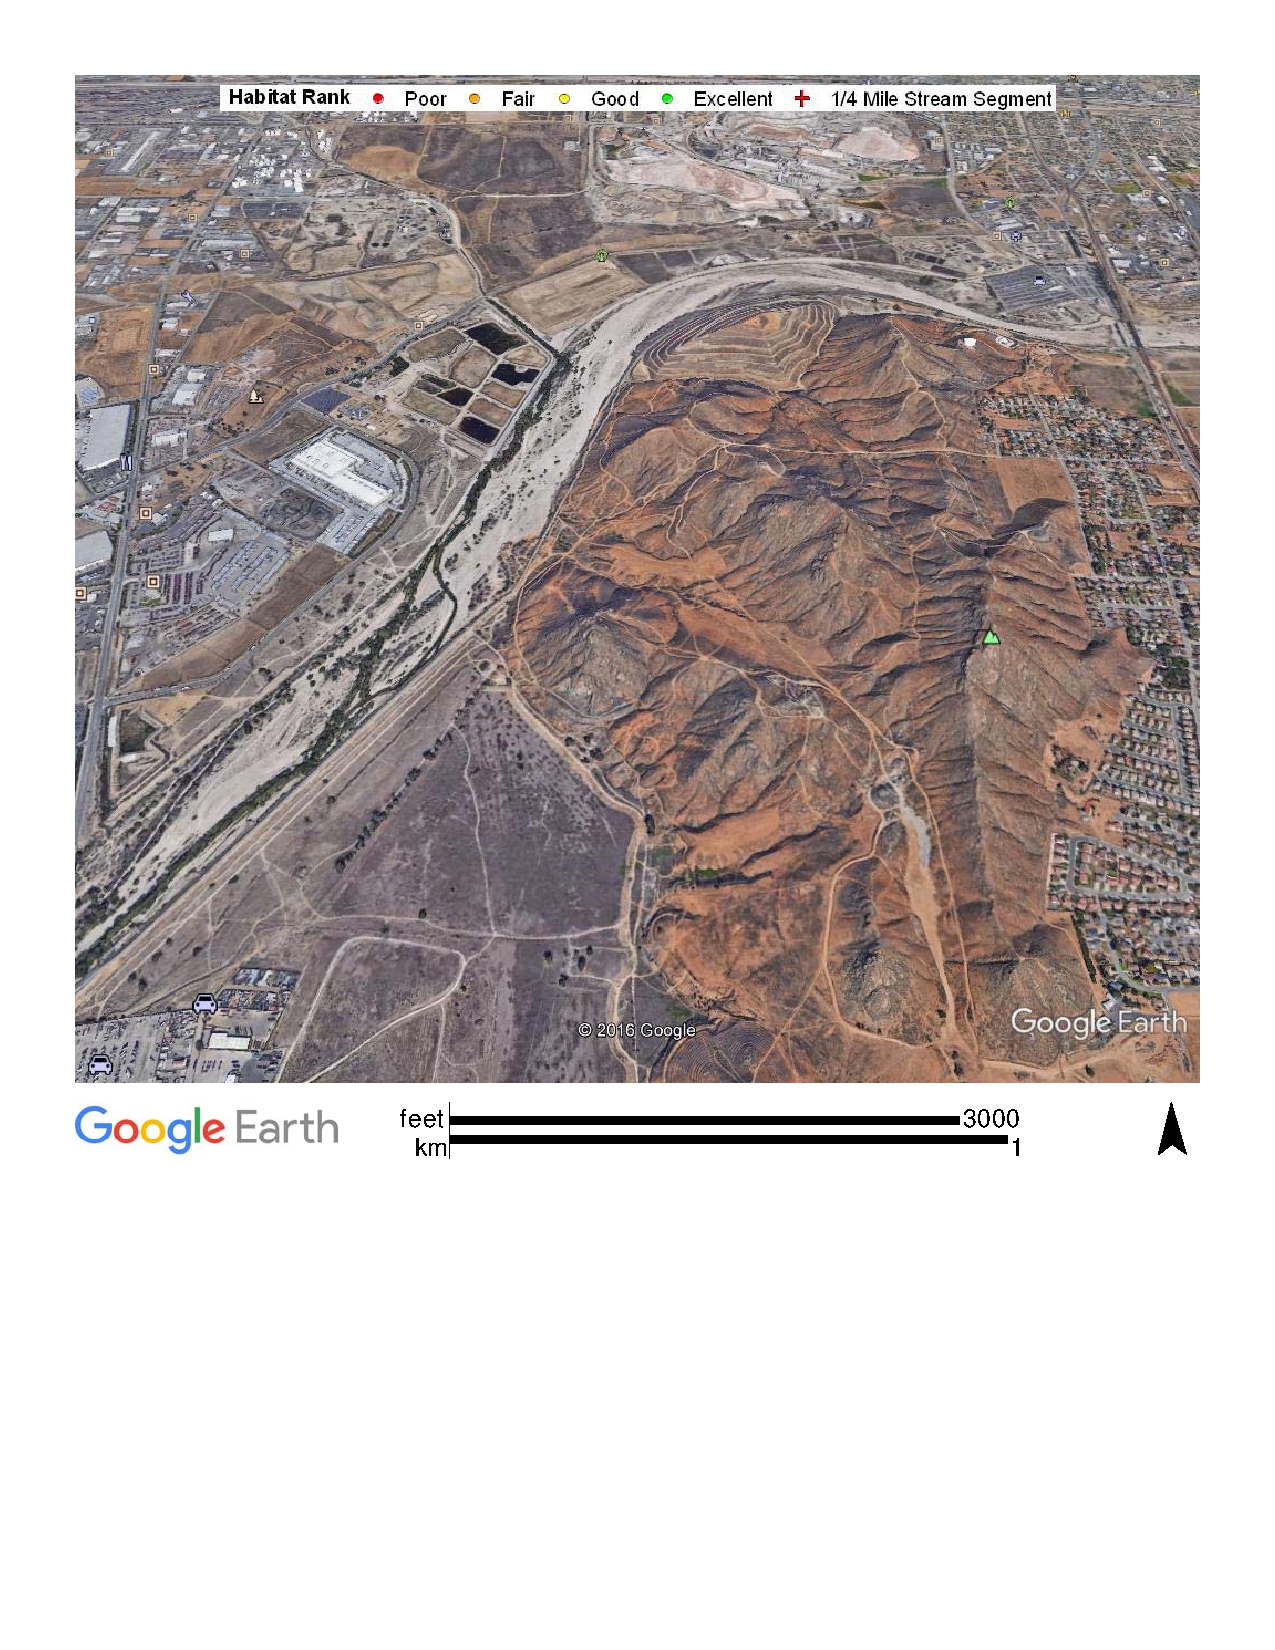
\includegraphics[width=1.00\textwidth]{Figures/SantaAna_SatelliteImage}
\caption{Google Earth --THIS IS HOW YOU DO A CAPTION IN CASE WE NEED IT}
\label{SAR_Image}
\end{figure}

\subsection{Field Methods}
The collection of data on the algae abundance, sediment type, vegetation canopy cover, 
and temperature of the Santa Ana River was done along the section of the river described
in the site description section on September 20th, 2016, from 1pm to 3:30pm.

9 measurements of each parameter were taken at Sites 4, 3, and 2, for a total of 27 measurements. 
At each site, beginning at Site 4, the following procedures were followed: 

1)A spot was chosen along the right bank. Each of the parameters were then measured.

2)For estimating algae abundance, we placed the 30  x 30 cm quadrat above the river bed and estimated
the percent that was covered by algae to the nearest 10 percent.

3)The sediment type of the site was characterized as either fine or coarse based on the grain size of the 30x30cm section of stream bed covered by the quadrat as either fine or coarse. Coarse substrate was classified as anything larger than pebbles or sand, that is, larger than 6.5cm. If more than half of the area covered by the quadrat was coarse substrate, or fine substrate, the area was characterized as such respectively.

4)Canopy cover was measured from the same position as the algae by holding spherical canopy densiometer above water at elbow’s length. Based on how many of the 15 intersections on the densiometer reflected overhead canopy, cover was then quantified on a 0-15 scale, 0 being the no canopy cover and 15 being full cover.

5)To measure temperature, we submerged the analog thermometer underwater and recorded the temperature in degrees Celsius.

6)Qualitative aspects of the river, such as presence of a pool or of logs, were also noted at each measurement spot.

7)Each measurement was then also taken at the middle of the river and the left bank of the cross-section. 

8)Steps 1)-7) Were repeated at two cross-sections between 0 and 10 meters downstream both chosen using a random number generator for a total of 3 cross-sections along a possible total length of 20 meters, and 3 measurements at each cross-section, for a total of 9 measurements per site. 


Steps 1)-8) were repeated at each Site, moving upstream from 4 to 2, for a total of 27 measurements of each parameter.


\subsection{Statistical Methods}

After conducting our fieldwork, we imported our data in rstudio and generated summary statistics using the following code: 
\begin{Schunk}
\begin{Sinput}
> updateddata= "/home/CAMPUS/fcl02013/Santa-Ana-Sucker-Recovery/Data/Data_TUES_1/updatedtemps.csv"
> importupdated=read.csv(updateddata)
\end{Sinput}
\end{Schunk}
=======
After conducting our fieldwork, we will enter our data in rstudio. We will produce linear regressions of temperature vs algae abundance. We will producelinear regressions of canopy cover vs algae abundance. We will produce linear regressions of canopy cover vs temperature. We will create ANOVA or t-tests of bed composition vs. algae abundance. We will then analyze our data and write a project report 4-5 pages long with pictures and figures. We should hopefully be able to draw conclusions about canopy cover, temperature, and stream bed compositions effect on algae abundance. In qualitative terms, we will synthesize our results with the fish videography team and state whether our observed relationship between stream conditions and algae abundance matches the frequency of their fish observations.
The following code was used to generate summary statisitics. 
INSERT CODE FOR SUMMARY STATISTICS
>>>>>>> f31b8abefbb905befede6108d156a650b766b1ff

Note that *Temp\_x* entries were borrowed with permission from Sophie and Nicole's dataset. We also created a "Site\_New" field so that our naming conventions whould be consistant with other teams. We then used rstudio to generate the following descriptive statisitcs:  
linear regression of temperature range vs algae abundance
linear regression of canopy cover vs algae abundance
ANOVA of bed composition vs. algae abundance
ANOVA of site location vs. algae abundance
For each of these statistical comparisons, we tested whether we could reject the null hypothesis, and if yes, discuss the implications of those findings. Our results are summarized in the following section. 
\section{Results and Discussion}

The temperature data we collected with an analogue thermometer was too coarse to really be useful, because we took all our measurements in one afternoon and could only take temperature measurments at a resolution of whole degrees celsius. For that reason, we instead used WED1 team's temperature data. The following is a plot of algae abundance as a function of range of temperature (*C) experienced at each site. 
<<<<<<< HEAD
\begin{knitrout}
\definecolor{shadecolor}{rgb}{0.969, 0.969, 0.969}\color{fgcolor}\begin{kframe}
\begin{alltt}
\hlkwd{plot}\hlstd{(importupdated}\hlopt{$}\hlstd{Temp_range,importupdated}\hlopt{$}\hlstd{Algae,} \hlkwc{ylab}\hlstd{=}\hlstr{"Algae Abundance (% cover)"}\hlstd{,}\hlkwc{xlab}\hlstd{=}\hlstr{"Temperature (*C)"}\hlstd{,}\hlkwc{main} \hlstd{=}\hlstr{"Temperature as a predictor of Algae Abundance"}\hlstd{,}\hlkwc{las}\hlstd{=}\hlnum{1}\hlstd{)}
\hlkwd{abline}\hlstd{(}\hlkwd{lm}\hlstd{(Algae}\hlopt{~}\hlstd{Temp_range,importupdated))}
\end{alltt}
\end{kframe}
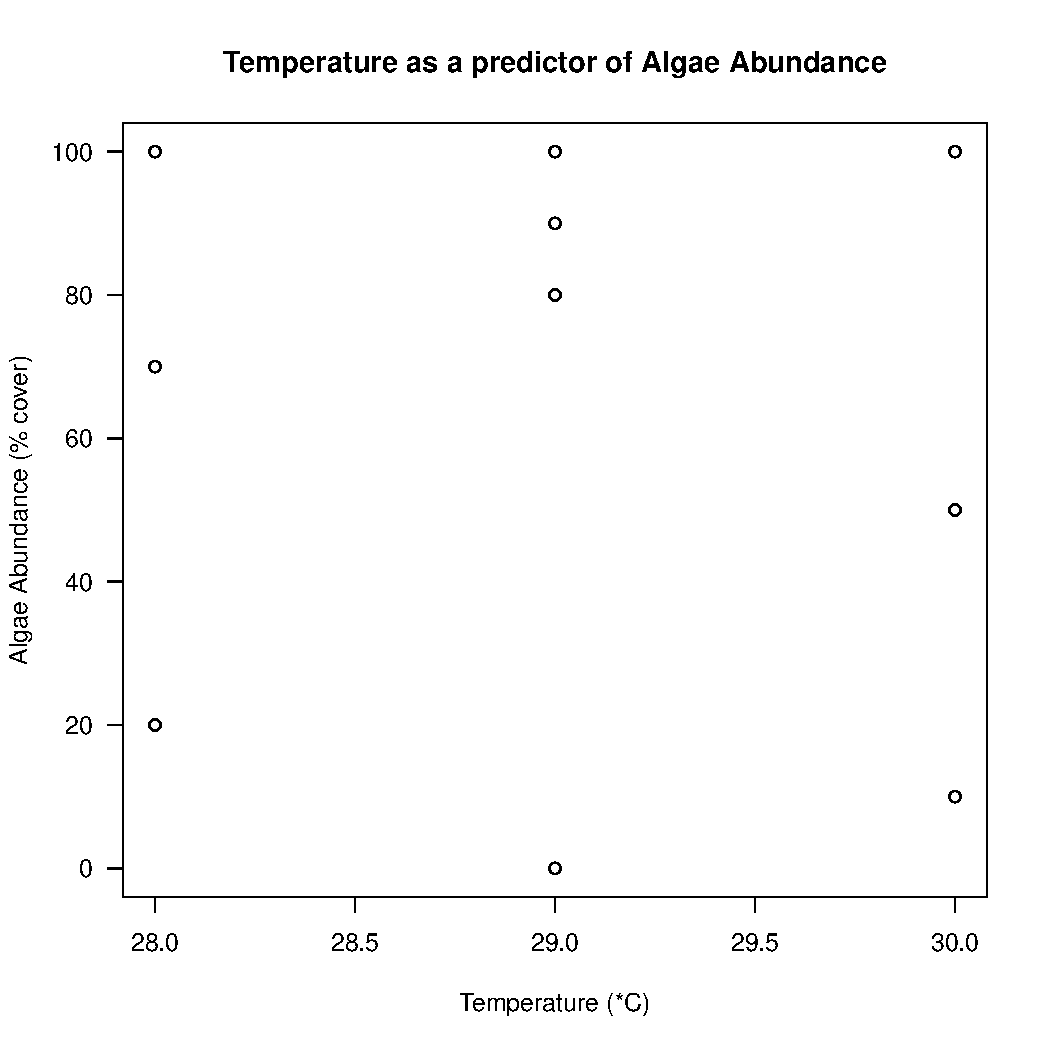
\includegraphics[width=\maxwidth]{figure/unnamed-chunk-2-1} 

\end{knitrout}
<<<<<<< HEAD
While using our absolute temperature data as a predictor of algae abundance yielded p-value: 0.446 (cannot reject null hypothesis), using the other teams's temperature d range data yilded the much better p-value of 3.49e-05. There is a strong nonrandom relationship between the range of temperatures a site experiences and the abundance of algae. However, with an Adjusted R-squared of only 0.4826, there are clearly other important variables at work as well. We find that higher variation in water temperatures generally coorelates to higher algae abundance. 
\begin{knitrout}
\definecolor{shadecolor}{rgb}{0.969, 0.969, 0.969}\color{fgcolor}\begin{kframe}
\begin{alltt}
\hlkwd{plot}\hlstd{(importupdated}\hlopt{$}\hlstd{Canopy,importupdated}\hlopt{$}\hlstd{Algae,} \hlkwc{ylab}\hlstd{=}\hlstr{"Algae Abundance (% cover)"}\hlstd{,}\hlkwc{xlab}\hlstd{=}\hlstr{"Canopy Cover Index"}\hlstd{,}\hlkwc{main} \hlstd{=}\hlstr{"Canopy Cover as a predictor of Algae Abundance"}\hlstd{,}\hlkwc{las}\hlstd{=}\hlnum{1}\hlstd{)}
\hlkwd{abline}\hlstd{(}\hlkwd{lm}\hlstd{(Algae}\hlopt{~}\hlstd{Canopy,importupdated))}
\end{alltt}
\end{kframe}
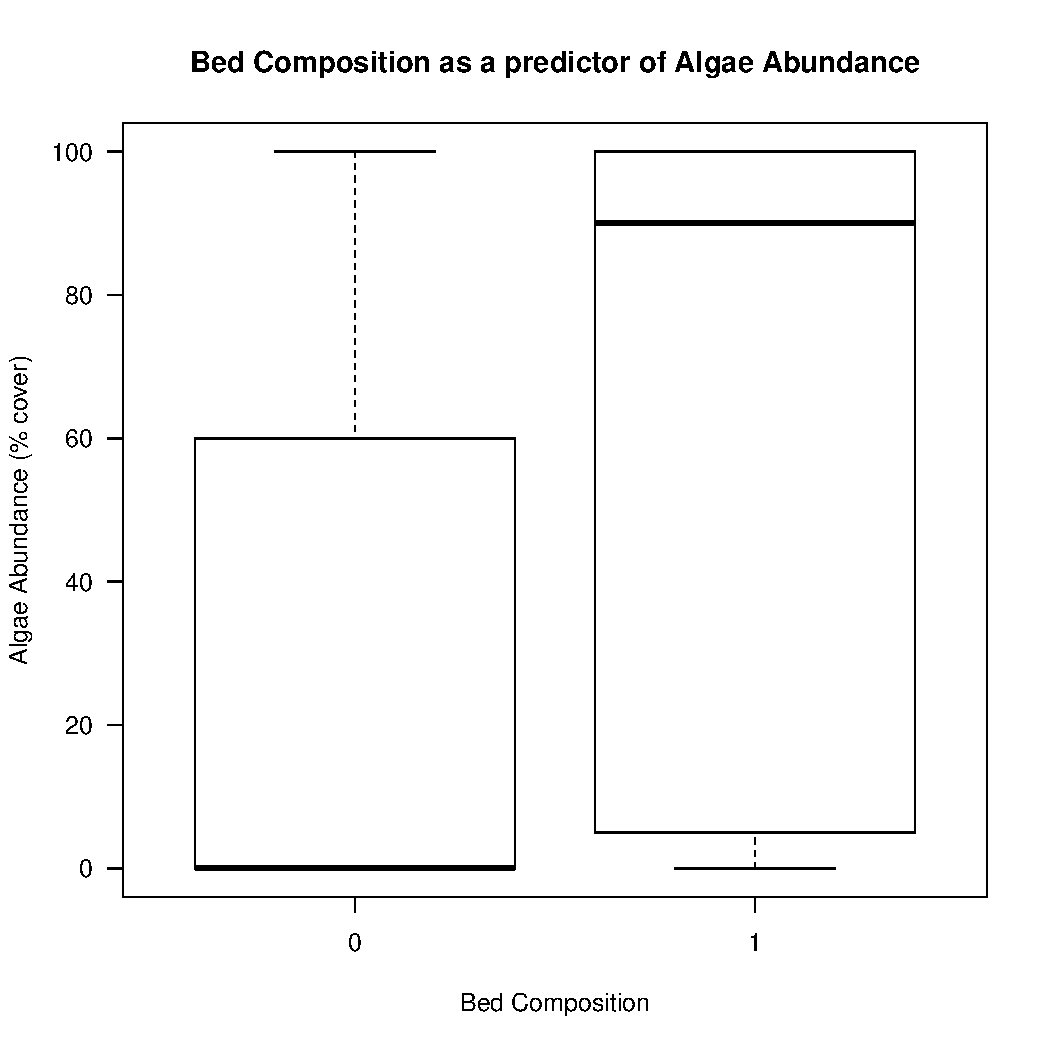
\includegraphics[width=\maxwidth]{figure/unnamed-chunk-3-1} 

\end{knitrout}
Canopy Cover was a very poor predictor of Algae Abnundance, with no predictive value. A linear regression yielded p-value: 0.3339, so we cannot reject the null hypothesis.
\begin{knitrout}
\definecolor{shadecolor}{rgb}{0.969, 0.969, 0.969}\color{fgcolor}\begin{kframe}
\begin{alltt}
\hlkwd{boxplot}\hlstd{(Algae}\hlopt{~}\hlstd{Sediment,importupdated,} \hlkwc{ylab}\hlstd{=}\hlstr{"Algae Abundance (% cover)"}\hlstd{,}\hlkwc{xlab}\hlstd{=}\hlstr{"Bed Composition"}\hlstd{,}\hlkwc{main} \hlstd{=}\hlstr{"Bed Composition as a predictor of Algae Abundance"}\hlstd{,}\hlkwc{las}\hlstd{=}\hlnum{1}\hlstd{)}
\end{alltt}
\end{kframe}
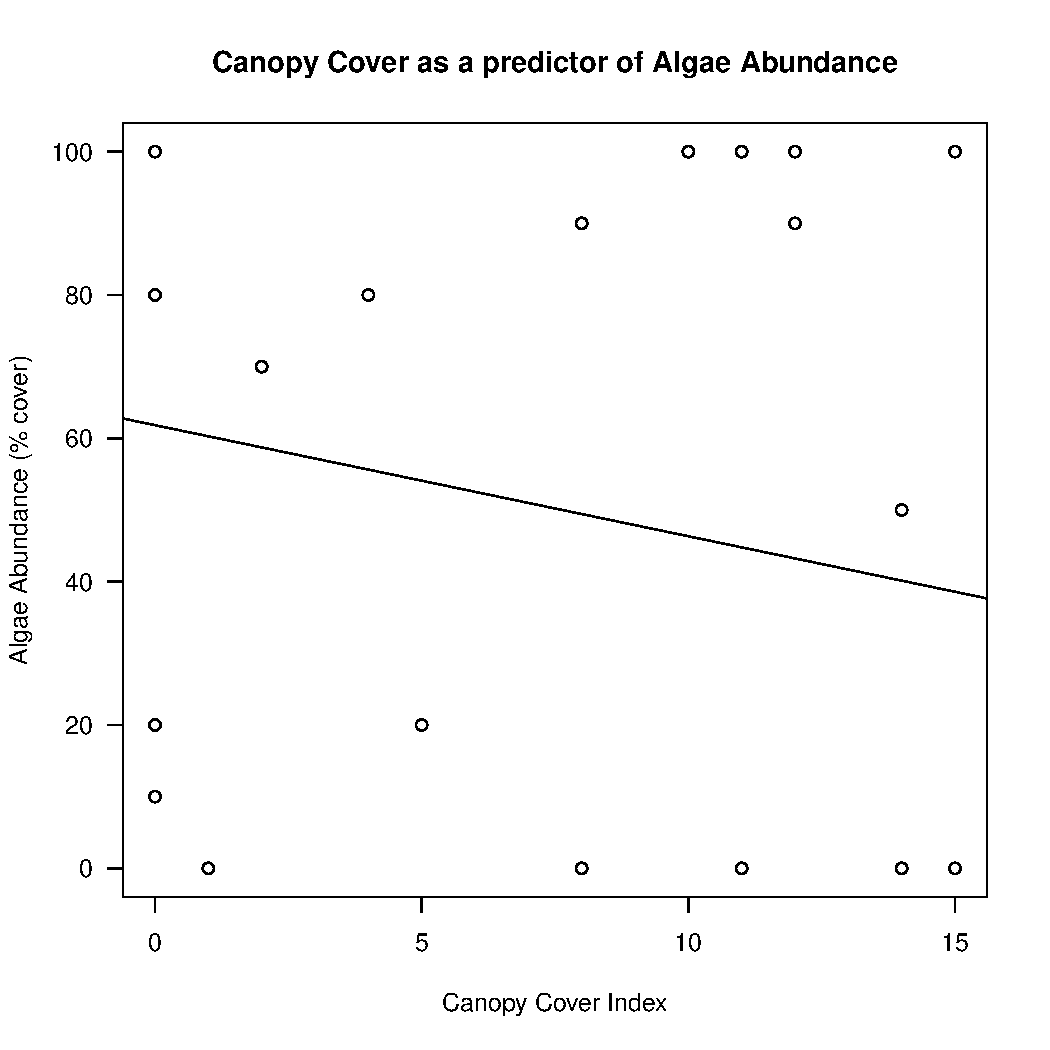
\includegraphics[width=\maxwidth]{figure/unnamed-chunk-4-1} 

\end{knitrout}
Bed composition did have a stronger relationship with Alage Abanundance, as shown in the figure above. 0 = fine sediment, while 1 = coarse sediment. Our P value=0.0643 which means we cannot reject null hypothesis, but only barely. This indicates that there is probably some relationship between algae cover and sediment composition of the stream bed, and this should be examined in future. In general, alage seem to perhaps prefer coarser sediment. 
\begin{figure}
\begin{knitrout}
\definecolor{shadecolor}{rgb}{0.969, 0.969, 0.969}\color{fgcolor}\begin{kframe}
\begin{alltt}
\hlkwd{boxplot}\hlstd{(Algae}\hlopt{~}\hlstd{Site_new,importupdated,} \hlkwc{ylab}\hlstd{=}\hlstr{"Algae Abundance (% cover)"}\hlstd{,}\hlkwc{xlab}\hlstd{=}\hlstr{"Site name"}\hlstd{,}\hlkwc{main} \hlstd{=}\hlstr{"Reach Site as a predictor of Algae Abundance"}\hlstd{,}\hlkwc{las}\hlstd{=}\hlnum{1}\hlstd{)}
\end{alltt}
\end{kframe}
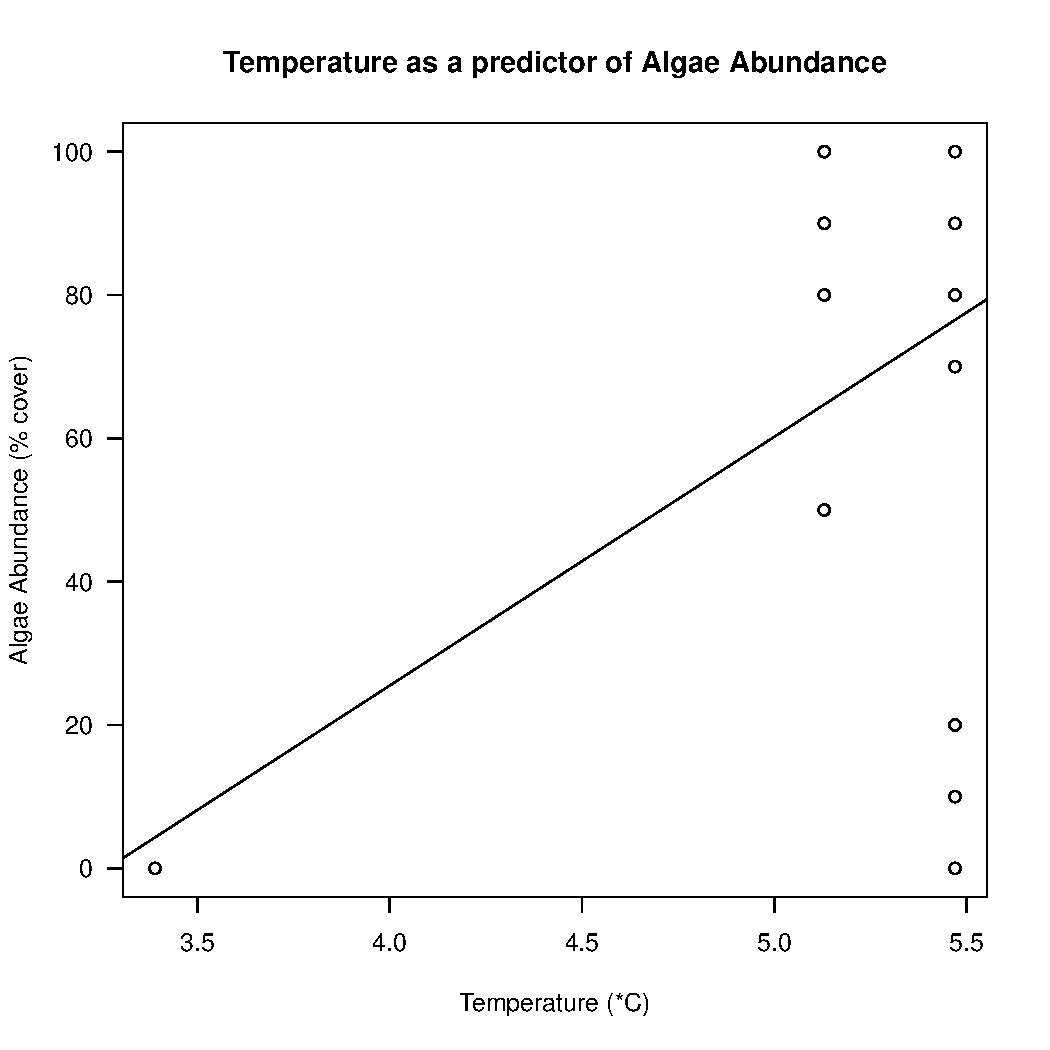
\includegraphics[width=\maxwidth]{figure/unnamed-chunk-5-1} 

\end{knitrout}
\end{figure}

As a control, we also analyzed to what extend Reach Site alone could predict Algae Abundance. Our ANOVA test yielded p-value: 0.008176 which means the reach of the river studied is alone one of our best predictors of algae abundance, second only to temperature variation. However, our temperature variation data was merged with our algae data after the fact, and for each site, all measurements were assigned the same temp_range value. Therefore, the high predictive value of temp_range could be just an artifact of that methodological decision. However, temperature variations p-value was over 2 orders of magnitude smaller than Reach Site alone (3.49e-05 vs. 8.17e-03 respectively), so it remains thoroughly plausible that water temperature variation is predictor of algae abundance independent of site variation. Because of our experiemental design, it is unfortunately impossible to control by site for temperature variation and see if the relationship remains robust. This should be examined in future work. 
=======
\begin{Schunk}
\begin{Sinput}
> plot(importupdated$Temp_range,importupdated$Algae, ylab="Algae Abundance (% cover)",xlab="Temperature (*C)",main ="Temperature as a predictor of Algae Abundance",las=1)
> abline(lm(Algae~Temp_range,importupdated))
\end{Sinput}
\end{Schunk}
<<<<<<< HEAD
While using our absolute temperature data as a predictor of algae abundance yielded p-value: 0.446 (cannot reject null hypothesis), using the other teams's temperature d range data yilded the much better p-value of 3.49e-05. There is a strong nonrandom relationship between the range of temperatures a site experiences and the abundance of algae. However, with an Adjusted R-squared of only 0.4826, there are clearly other important variables at work as well. We find that higher variation in water temperatures generally coorelates to higher algae abundance. 
\begin{Schunk}
\begin{Sinput}
> plot(importupdated$Canopy,importupdated$Algae, ylab="Algae Abundance (% cover)",xlab="Canopy Cover Index",main ="Canopy Cover as a predictor of Algae Abundance",las=1)
> abline(lm(Algae~Canopy,importupdated))
\end{Sinput}
\end{Schunk}
Canopy Cover was a very poor predictor of Algae Abnundance, with no predictive value. A linear regression yielded p-value: 0.3339, so we cannot reject the null hypothesis.
\begin{Schunk}
\begin{Sinput}
> boxplot(Algae~Sediment,importupdated, ylab="Algae Abundance (% cover)",xlab="Bed Composition",main ="Bed Composition as a predictor of Algae Abundance",las=1)
\end{Sinput}
\end{Schunk}
Bed composition did have a stronger relationship with Alage Abanundance, as shown in the figure above. 0 = fine sediment, while 1 = coarse sediment. Our P value=0.0643 which means we cannot reject null hypothesis, but only barely. This indicates that there is probably some relationship between algae cover and sediment composition of the stream bed, and this should be examined in future. In general, alage seem to perhaps prefer coarser sediment. 
\begin{Schunk}
\begin{Sinput}
> boxplot(Algae~Site_new,importupdated, ylab="Algae Abundance (% cover)",xlab="Site name",main ="Reach Site as a predictor of Algae Abundance",las=1)
\end{Sinput}
\end{Schunk}
As a control, we also analyzed to what extend Reach Site alone could predict Algae Abundance. Our ANOVA test yielded p-value: 0.008176 which means the reach of the river studied is alone one of our best predictors of algae abundance, second only to temperature variation. However, our temperature variation data was merged with our algae data after the fact, and for each site, all measurements were assigned the same temp\_range value. Therefore, the high predictive value of temp\_range could be just an artifact of that methodological decision. However, temperature variations p-value was over 2 orders of magnitude smaller than Reach Site alone (3.49e-05 vs. 8.17e-03 respectively), so it remains thoroughly plausible that water temperature variation is predictor of algae abundance independent of site variation. Because of our experiemental design, it is unfortunately impossible to control by site for temperature variation and see if the relationship remains robust. This should be examined in future work. 
>>>>>>> 01ba632b1f399fbbda3be47972e667807001f8ce
=======
>>>>>>> 4d209e808746e9ef3b8e29225dd53b12dcd8e799

The temperature data suggests... (Figure \ref{Temp}).

\begin{figure}
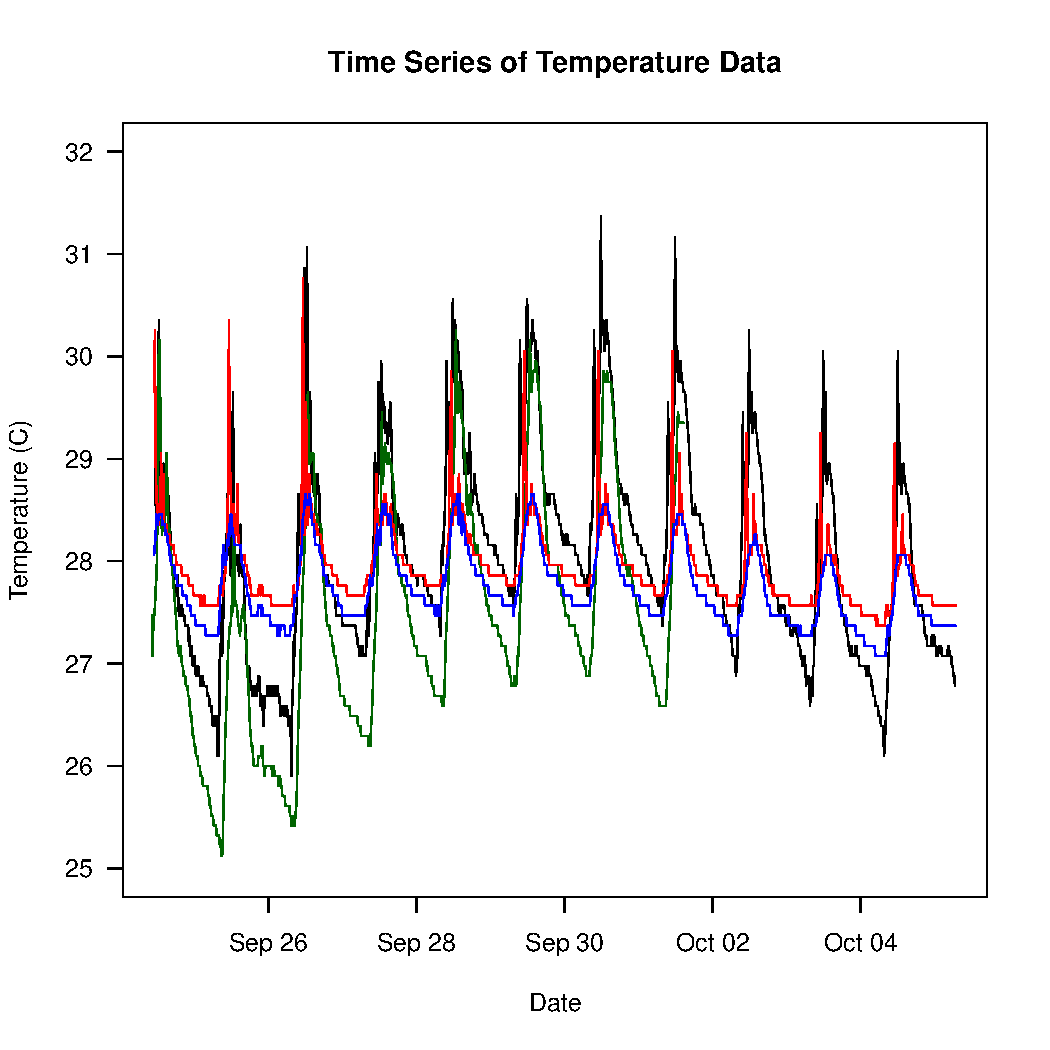
\includegraphics{Figures/Temp}
\caption{Temperature time...}
\label{Temp}
\end{figure}

\subsection{Discussion}

Water temperature vs Algae Abundance: Our temperature data is coarse, measured in whole degrees, and has no predictive value. Data collection was limited to of one afternoon. The P-value was 0.446 for a linear regression testing correlation between water temperature and algae abundance. 
We cannot reject the null hypothesis of no relationship between the two parameters.
However, Fish and Wildlife Service employee, Kai Pelenscar, suggested that temperature variation, rather than absolute temperature, might be the  controlling factor of algae abundance. 


We borrowed data from N. Larson and Sophie J., and assigned their measured ranges of temp to each site. We redid our linear regression with temp range at each site as the predictor variable, and this time got a very strong relationship, with a p-value: 3.49e-05.


There is a strong nonrandom relationship between the range of temperatures a site experiences and the abundance of algae. However, with an adjusted R-squared of only 0.4826, there are clearly other important variables at work.


Canopy Cover was a very poor predictor of Algae Abundance, with no predictive value. A linear regression yielded p-value: 0.3339, so we cannot reject the null hypothesis of no difference.


Bed composition did have a stronger relationship with Alage Abundance, as sjhown in the figure above. 0 = fine sediment, while 1 = coarse sediment. Our Pr(>F)=0.0643 which means we cannot reject null hypothesis, but only barely. This indicates that there is probably some relationship between algae cover and sediment composition of the stream bed, and this should be examined in future.

\section{Conclusion and Recommendations}
There is a statistically significant variation of algae abundance between the 3 sites examined in our study. Some measurements showed up to 100 percent algae cover, while others exhibited none. This variation suggests the possibility that algae may be controlled by specific variables. We tested whether water temperature, water temperature variation, canopy cover, or stream bed composition could explain these variations. Of these possible causal factors, we found the strongest evidence for higher water temperature variation exerting a positive effect of algae abundance. The relationship between algae cover and streambed sediment composition of the stream bed was not statistically significant at the 95 percent level, but did tentatively suggest that algae may prefer coarse sediment. Red Algae in the Santa Ana River has a highly unequal distribution, that appears to be controlled in part by water temperature variation, with a possible small contribution of streambed sediment composition. 
Our exploratory study is one of the first to examine what variables may control red algae's distribution in the Santa Ana River. While the limited scope of this research eliminated the possibility of conclusive findings, we can suggest promising areas for further research. Future studies should more systematically examine the relationship between temporal variability in water temperature and algae abundance. Sediment type should be assigned to narrow categories such as silt, sand, gravel, and cobbles rather than simply being tagged as fine or coarse. More than 3 reaches/sites should be used. Most importantly, red algae’s co-occurrence with the federally endangered Santa Ana sucker should be examined. These improvements on our experiment will yield a much better idea of what factors control red algae’s distribution in the Santa Ana River, and create a statistically supported foundation for considering the algae’s effect on Santa Ana Suckers. 

\end{document}


